\documentclass[../main.tex]{subfiles}
\begin{document}
\section{Introduction}
\label{sec:intro}
\begin{figure}[h]
    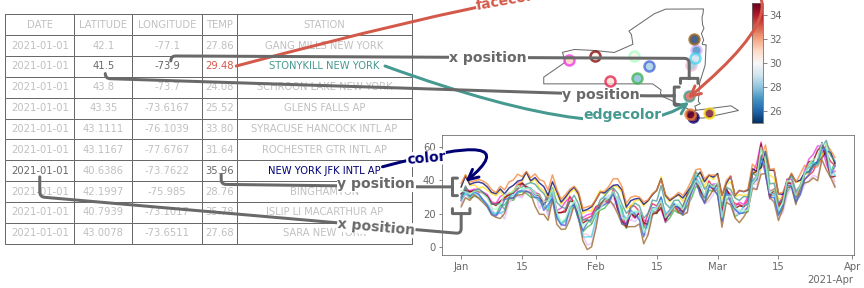
\includegraphics[width=1\textwidth]{figures/intro/functions.png}
    \caption{Visualizations are made up of transformations from data into visual representation. These functions transform individual data values to visual representation, such as date to x position or latitude to y position. These functions are composed into the assembly of all these transformations into a visual mark, such as a line or point. %%% break this out into seperate sentences to break 
    The same variable can be mapped in different ways, for example line is mapped to a color in the scatter plot and to y position in the line plot.}
    \label{fig:intro:artist}
\end{figure}
Visualization is the transformation of data into visual representation. As illustrated by \autoref{fig:intro:artist}, these translations are both at the level of the individual variable and the entire record. In the case of the scatter plot, the latitude and longitude are encoded as the x and y position, respectively, while the temperature and station are represented by the face and edge colors. A row in the table is collectively encoded as a point mark. None of these encodings are fixed, as evidenced by temperature being translated into the y value in the case of the line plot. The station is now the source of the color of the entire line, and the date is the x position. As with scatter, the encodings of the individual transformations, which again are on values from the same record in the table, are composited into a line mark. It is these raw transformations from data space to visualization space that are implemented by building block level visualization libraries, named as such because the functions provided by the library can be composited in any number of ways to yield visualizations \cite{wongsuphasawatNavigatingWideWorld2021}. We propose that like physical building blocks, building block libraries must provide a collection of well defined pieces that can be composed in whichever ways the blocks fit together. We specify that a valid visualization block is a structure preserving transformation from data to visual space, and we define structure in terms of \textit{continuity} and \textit{equivariance}. We then use this model to develop a design specification for the components of a building block visualization library. The notion of self contained, inherently modular, building blocks lends itself naturally to a functional paradigm of visualization \cite{hughesWhyFunctionalProgramming1989}. We adopt a functional model for a redesign because the lack of side effects means functional architecture can be evaluated for correctness, functional programs tend to be shorter and clearer, and are well suited to distributed, concurrent, and on demand tasks\cite{huHowFunctionalProgramming2015}.

This work is strongly motivated by the needs of the Matplotlib\cite{hunterMatplotlib2DGraphics2007,hunterArchitectureOpenSource} visualization library. One of the most widely used visualization libraries in Python, since 2002 new components and features have been added in a some what adhoc, sometimes hard to maintain, manner. Particularly, each new component carries its own implicit notion of how it believes the data is structured-for example if the data is a table, cube, image, or network - that is then expressed in the API for that component. In turn, this yields an inconsistent API for interfacing with the data, for example when  updating streaming visualizations or constructing dashboards\cite{a.sarikayaWhatWeTalk2019}. This entangling of data model with visual transform also yields inconsistencies in how visual component transforms, e.g. shape or color, are supported. We propose that these issues can be ameliorated via a redesign of the functions that convert data to graphics, named \textit{Artists} in Matplotlib, in a manner that reliably enforces \textit{continuity} and \textit{equivariance} constraints. We evaluate our functional model by implementing new artists in Matplotlib that are specified via \textit{equivariance} and \textit{continuity} constraints. We then use the common data model introduced by the model to demonstrate how plotting functions can be consolidated in a way that makes clear whether the difference is in expected data structure, visual component encoding, or the resulting graphic. 

\section{Background}
There are many formalisms of the notion that visualization is structure preserving maps from data to visual representation, and many visualization libraries that attempt to preserve structure in some manner; this work bridges the formalism and implementation in a functional manner with a topological approach at a building blocks library level to propose a new model of the constraints visual transformations must satisfy such that they can be composed to produce visualize representations that can be considered equivalent to the data being represented.

\subsection{Structure:}
\label{sec:intro:structure}
Visual representations of data, by definition, reflect something of the underlying structure and semantics\cite{friendlyBriefHistoryData2008}, whether through direct mappings from data into visual elements or via figurative representations that have meaning due to their similarity in shape to external concepts \cite{byrneAcquiredCodesMeaning2016}. The components of a visual representation were first codified by Bertin\cite{bertinSemiologyGraphicsDiagrams2011a}, who introduced a notion of structure preservation that we formally describe in terms of \textit{equivariance} and \textit{continuity}. 
 
\begin{figure}[H]
        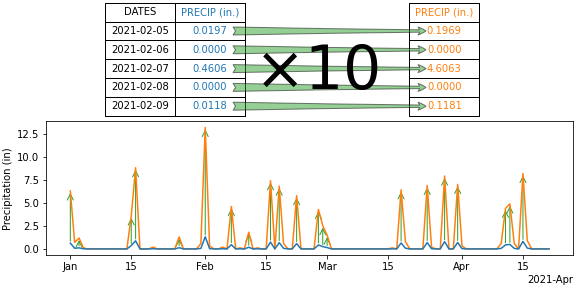
\includegraphics[width=1\columnwidth]{figures/intro/equivariant.png}
        \caption{The data in blue is scaled by a factor of two, yielding the data in orange. To preserve \textit{equivariance}, the blue line plot representation of the unscaled data is also scaled by a factor of two, yielding the orange line plot that is equivalent to the scaled data.}
        \label{fig:intro:equivariance}
\end{figure}
Bertin proposes that there are classes of visual encodings-such as position, shape, color, and texture-that when mapped to from specific types of measurement, quantitative or qualitative, will preserve the properties of that measurement type. For example, in \autoref{fig:intro:equivariance}, the data and visual representation are scaled by equivalent factors of two, resulting in the change illustrated in the shift from blue to orange data and lines. The idea of equivariance is formally defined as the mapping of a binary operator from the data domain to the visual domain in Mackinlay's \textit{A Presentation Tool}(APT) model\cite{mackinlayAutomatingDesignGraphical1986, mackinlayAutomaticDesignGraphical1987}. The algebraic model of visualization proposed by Kindlmann and Scheidegger uses equivariance to refer generally to invertible binary transformations\cite{kindlmannAlgebraicProcessVisualization2014}, which are mathematical groups \cite{shadrachIntroductionGroups2017}. Our model defines \textit{equivariance} in terms of monoid actions, which are a more restrictive set than all binary operations and more general than groups. As with the algebraic model, our model also defines structure preservation as commutative mappings from data space to representation space to graphic space, but our model uses topology to explicitely include continuity.

\begin{figure}[H]
    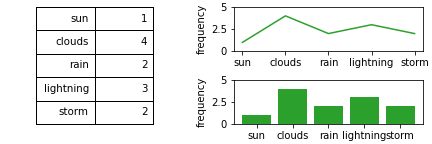
\includegraphics[width=1\textwidth]{figures/intro/continuity.png}
    \caption{The line plot does not preserve \textit{continuity} because it implies that the average temperature at each station lie along a 1D continuous line, while the bar plot preserves \textit{continuity} by representing the average temperatures at each station as the discrete values they are.}
    \label{fig:intro:continuity}
\end{figure}
Bertin proposes that the visual encodings be composited into graphical marks that match the \textit{continuity} of the data - for example discrete data is a point, 1D continuous is the line, and 2D data is the area mark. In \autoref{fig:intro:continuity}, the line plot does not preserve continuity because the line connecting the discrete categories implies that the frequency of weather events is sampled from a continuous interval and the categories are points on that interval. But, when the continuity is preserved, as in the bar chart, then the graphic has not introduced new structure into the data. 

\begin{mdframed}[roundcorner=10pt, frametitle=Structure, frametitlerule=true, frametitlebackgroundcolor=gray!10]
    \begin{description}
        \item[\textbf{continuity}] How records in the dataset are connected to each other, e.g. discrete rows, neworked nodes, points on a continuous surface
        \item[\textbf{equivariance}] if an action is applied to the data or the graphic--e.g. a rotation, permutation, translation, or rescaling-- there must be an equivalent action applied on the other side of the transformation. 
    \end{description}
\end{mdframed}

The notion that a graphic should be equivalent to the data has been expressed in a variety of ways. Informally, Norman's Naturalness Principal\cite{NaturalnessPrincipleInfoVis} states that a visualization is easier to understand when the properties of the visualization match the properties of the data. This principal is made more concrete in Tufte's concept of graphical integrity, which is that a visual representation of quantitative data must be directly proportional to the numerical quantities it represents (Lie Principal), must have the same number of visual dimensions as the data, and should be well labeled and contextualized, and not have any extraneous visual elements\cite{tufteVisualDisplayQuantitative2001}. expressing, as defined by Mackinlay, is a measure how much of the mathematical structure in the data that can be expressed in the visualizations; for example that ordered variables can be mapped into ordered visual elements. We propose that a graphic is an equivalent representation of the data when \textit{continuity} and \textit{equivariance} are preserved.



\subsection{Tools}
\label{sec:intro:data:tools}

\begin{figure}[H]
    \begin{subfigure}{.3\textwidth}
        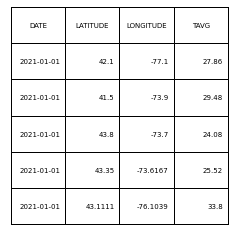
\includegraphics[width=1\textwidth]{figures/intro/table.png}
    \end{subfigure}
    \begin{subfigure}{.3\textwidth}
        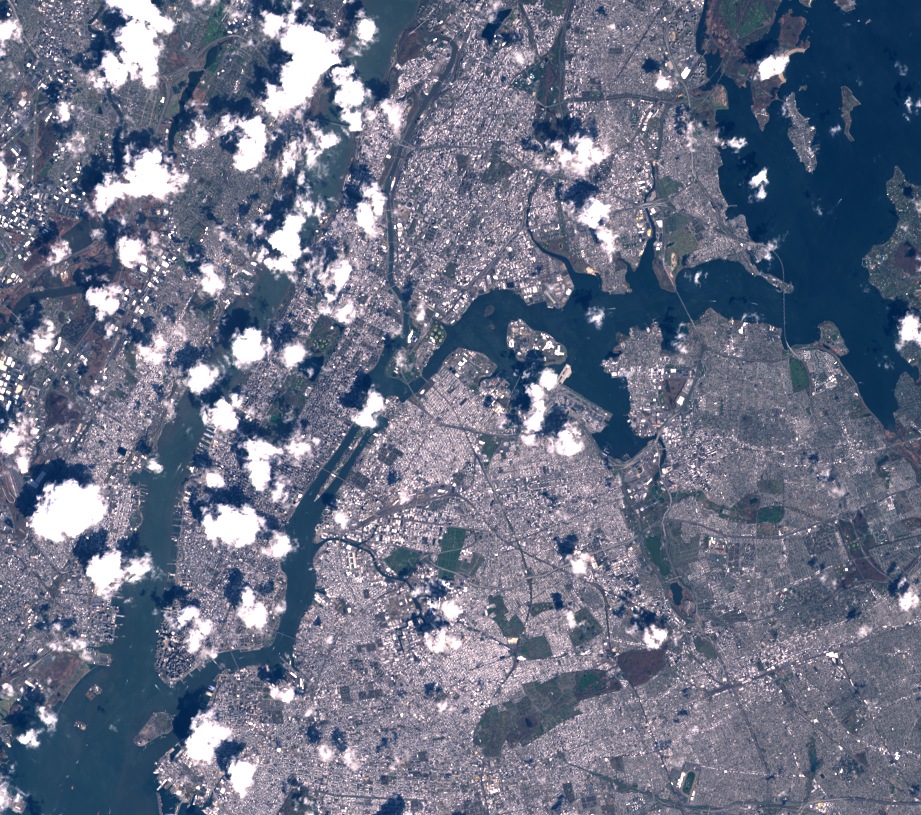
\includegraphics[width=1\textwidth]{figures/intro/landsat.png}
    \end{subfigure}
    \begin{subfigure}{.3\textwidth}
        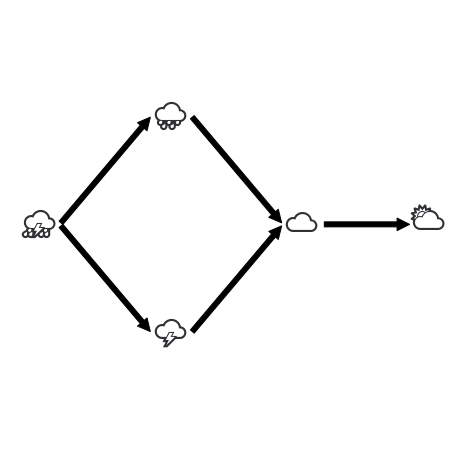
\includegraphics[width=1\textwidth]{figures/math/graph.png}
    \end{subfigure}
    \caption{Visualization libraries, especially ones tied to specific domains, tend to be architectured around a core data structure, such as tables, images, or networks. }
    \label{fig:intro:data}
\end{figure}

One of the reasons we developed a new formalism rather than adopting the architecture of an existing library is that most information visualization software design patterns, as categorized by Heer and Agrawala\cite{HeerSoftware2006}, are tuned to very specific data structures. These libraries can often assume the expected data structure because they are domain specific, and that is the common data structure in that domain.  For users who generally work in one domain, such as the data, networks, or graphs shown in \autoref{fig:intro:data}, this well defined data space (and corresponding visual space\cite{chiTaxonomyVisualizationTechniques2000}) often yields a very coherent user experience\cite{heerDeclarative2010}. But, for developers who want to build new visualizations on top of these libraries, they must work around the existing assumptions, sometimes in ways that break the model the libraries are developed around. 


For example, many domain specific libraries integrate computation into the visualization, for example libraries based that assume all data is a relational database. This assumption is core to tools influenced by APT, such as Tableau\cite{StoltePolaris2002,hanrahanVizQL2006,MackinlayShowme2007} and the Grammar of Graphics\cite{wilkinsonGrammarGraphics2005}, such as ggplot\cite{wickhamGgplot2ElegantGraphics2016a}, protovis\cite{bostockProtoviz2009}, vega\cite{satyanarayanDeclarativeInteractionDesign2014} and altair\cite{vanderplasAltairInteractiveStatistical2018}. Since these libraries represent all data as a table, and computations on tables are fairly well defined\cite{ullmanFirstCourseDatabase2008}, they can include computations on the table with a fair bit of confidence that the computation is accurate. Since most computations are specific to domains, general purpose block libraries can not make this assumption; instead a goal of this model is to identify which computations are specifically part of the visual encoding - for example mapping data to a color-and which are manipulations on the data. Disentangling the computation from the visual transforms allows us to determine whether the visualization library needs to handle them or if they can be more efficiently computed by the data container.


A different class of user facing tools are those that support images, such as ImageJ\cite{schneiderNIHImageImageJ2012} or Napari\cite{nicholas_sofroniew_2021_4533308}. These tools often have some support for visualizing non image components of a complex data set, but mostly in service to the image being visualized. These tools are ill suited for general purpose libraries that need to support data other than images because the architecture is oriented towards building plugins into the existing system \cite{WritingPlugins} where the image is the core data structure. Even the digital humanities oriented ImageJ macro ImagePlot\cite{studiesCulturevisImageplot2021}, which supports some non-image aggregate reporting charts, is still built around image data as the primary input. The need to visualize and manipulate graphs has spawned tools like Gephi\cite{bastianGephiOpenSource2009}, Graphviz\cite{ellsonGraphvizOpenSource2002}, and Networkx\cite{HagbergExploringNetwork2008}. As with tables and images, extending network libraries to work with other types of data either require breaking their internal model of how data is structured and what transformations of the data are allowable or growing a model for other types of data structures alongside the network model. 


\begin{figure}[H]
    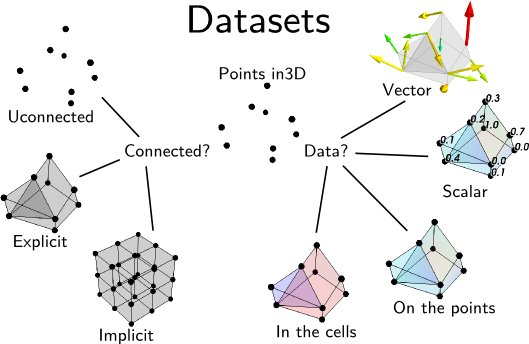
\includegraphics[width=1\textwidth]{figures/intro/dataset_diagram.png}
    \caption{One way to describe data is by the connectivity of the points in the dataset. A database for example is often discrete unconnected points, while an image is an implicitely connected 2D grid. This image is from the Data Representation chapter of the MayaVi 4.7.2 documentation.\cite{DataRepresentationMayavi}}
    \label{fig:intro:data:format}
\end{figure}
Many building block libraries carry multiple models of data internally because they cannot assume a data structure. Algorithms are designed such that the structure of data is assumed, as described in Tory and Möller's taxonomy \cite{ToryRethinkingVisualization2004}, and by definition building block libraries try to  provide the components to build any sort of visualization. Matplotlib, D3\cite{bostockDataDrivenDocuments2011}, and VTK \cite{hanwellVisualizationToolkitVTK2015,geveci2012vtk} and its derivatives such as MayaVi\cite{RamachandranMayaVI2011} and extensions such as ParaView\cite{ahrens2005paraview} and the infoviz themed Titan\cite{brianwylieUnifiedToolkitInformation2009}. Where GoG and ImageJ type libraries have coherant APIs for their visualization tools because the data structure is the same, the APIs for visualizations in Matplotlib, D3, and VTK are significantly dependent on the structure of the data it expects. VTK has codified this in terms of \textit{continuity} based data representations, as illustrated in figure~\ref{fig:intro:data:format}. This API choice can lead to visualizations that break \textit{continuity} when fed into visualizations with different assumptions about structure. The lack of consistent data model can also mean no consistent way of updating the data and therefore no way of guaranteeing that the views are in sync, in visualizations that consistent of multiple views of the same datasource, such as dashboards\cite{a.sarikayaWhatWeTalk2019,fewDashboardConfusionRevisited2007}. To resolve this issue, our functional model takes as input a structure aware data abstraction general enough to provide a common interface for many different types of visualization.

\subsection{Data}
\label{sec:intro_data}
One such general abstraction are fiber bundles, which Butler proposed as a core data structure for visualization because they encode data continuity separately from the variable properties and are flexible enough to support discrete and ND continuous datasets \cite{butlerVisualizationModelBased1989,butlerVectorBundleClassesForm1992}. 
Since Butler's model lacks a robust way of describing variables, we can encode a schema like description of the data in the fiber bundle by folding in Spivak's topological description of data types \cite{spivakDatabasesAreCategories2010,spivakSIMPLICIALDATABASES}. In this work we will refer to the points of the dataset as \textit{records} to indicate that a point can be a vector of heterogenous elements. Each \textit{component} of the record is a single object, such as a temperature measurement, a color value, or an image. We also generalize \textit{component} to mean all objects in the dataset of a given type, such as all temperatures or colors or images. The way in which these records are connected is the \textit{connectivity}, \textit{continuity}, or more generally \textit{topology}.

\begin{figure}[H]
    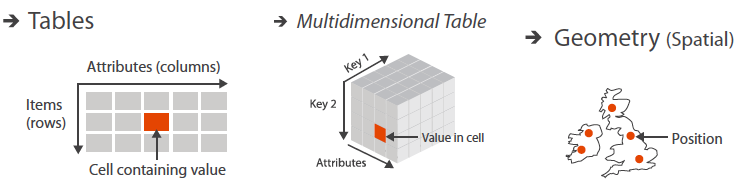
\includegraphics[width=1\textwidth]{figures/intro/munzner_datatypes.png}
    \caption{Values in a dataset have keys associated with them that describe where the value is in the dataset. These keys can be indexers or semantically meaningful;for example, in a table the keys are the variable name and the row ID. In the data cube,  the keys is the row, column, and cell ID, and in the map the key is the position in the grid. Image is figure 2.8 in Munzner's Visualization Analysis and Design\cite{munznerVisualizationAnalysisDesign2014}}
    \label{fig:intro:keys:values}
\end{figure}

The \textit{continuity} can often be described by some variables in the dataset; this is formalized Munzner's notion of metadata as \textit{keys} into the data structure that return associated \textit{values}\cite{munznerChDataAbstraction}. As shown in \autoref{fig:intro:keys:values}, keys can be labeled indexes, such as the attribute name and row ID, or physical entities such as locations on a map. We propose that information rich metadata are part of the components and instead the values are keyed on coordinate free structural ids. In contrast to Munzner's model where the semantic meaning of the key is tightly coupled to the position of the value in the dataset, our model considers keys to be a pure reference to topology. This allows the metadata to be altered, without imposing new semantics on the underlying structure, for example by changing the coordinate systems or time resolution. This value agnostic model also supports encoding datasets where there may be multiple independent variables - such as a measure of plant growth given variations in water, sunlight, and time - without having to assume any one variable is inducing the change in growth. For building block library developers, this means the components are able to fully traverse the data structures without having to know anything about the values or the semantic meaning of the structure. Since these components are by design \textit{equivariant} and \textit{continuity} preserving, domain specific library developers in different domains that both rely on the same continuity, for example 2D continuity, can then safely reuse the components to build tools that can safely make domain specific assumptions.

\subsection{Contribution}
The contribution of this work is 
\begin{enumerate}
  \item formalization of the topology preserving relationship between data and graphic via continuous maps \autoref{sec:math:graphic:base}
  \item formalization of property preservation from data component to visual representation as monoid action equivariant maps \autoref{sec:math:artist:nu}
  \item functional oriented visualization architecture built on the mathematical model to demonstrate the utility of the model \autoref{sec:math:artist:q}
  \item prototype of the architecture built on Matplotlib's infrastructure to demonstrate the feasibility of the model. \autoref{sec:math:code:artist}
\end{enumerate}
\end{document}